%
% Complete documentation on the extended LaTeX markup used for Insight
% documentation is available in ``Documenting Insight'', which is part
% of the standard documentation for Insight.  It may be found online
% at:
%
%     http://www.itk.org/

\documentclass{InsightArticle}


\usepackage{amsfonts}                 %Maths fonts
\usepackage{amssymb}                  %Maths symbols
\usepackage{listing}                  %Used for list of listings
\usepackage{listings}                 %List program code source
\usepackage{subfigure}                %For subfigures
\usepackage{color}                    %Allow color
\usepackage{fancyhdr}                 %Use headers and footers
\usepackage{graphicx}                 %Graphics
\usepackage{ccaption}
\usepackage{dsfont}
\usepackage[dvipdfm=true,
            bookmarks=true,
            bookmarksopen=true,
            bookmarksopenlevel=2,
            bookmarksnumbered=true,
            backref=section,
            colorlinks=true,
            linkcolor={blue},
            citecolor={blue},
            urlcolor={blue}]{hyperref}

%Allow code listings
%====================================================================
% Filename: listcode.tex
% Author: Daniel Mueller [d.mueller@qut.edu.au]
%--------------------------------------------------------------------
% Description: 
% Encapulates commands to list source code using the listings package.
% Also loads the [Shading]OpenGL language.
%--------------------------------------------------------------------
% Notes:
% - The listings package does not integrate well with the memoir class...
%	It may be necessary to delete the *.lol (local listing file) if an error
%   occurs during compilation.
%====================================================================              

%--------------------------------------------------------------------
% Define useful colours
\definecolor{listcomment}{rgb}{0.0,0.5,0.0}
\definecolor{listkeyword}{rgb}{0.0,0.0,0.5}
\definecolor{listnumbers}{gray}{0.65}
\definecolor{listlightgray}{gray}{0.955}
\definecolor{listwhite}{gray}{1.0}

%--------------------------------------------------------------------
% Configure C# listings
\newcommand{\listcsharp}
{
\lstset{frame = tb,
        framerule = 0.25pt,
        float,
        fontadjust,
        backgroundcolor={\color{listlightgray}},
        basicstyle = {\ttfamily\footnotesize},
        keywordstyle = {\ttfamily\color{listkeyword}\textbf},
        identifierstyle = {\ttfamily},
        commentstyle = {\ttfamily\color{listcomment}\textit},
        stringstyle = {\ttfamily},
        showstringspaces = false,
        showtabs = false,
        numbers = left,
        numbersep = 6pt,
        numberstyle={\ttfamily\color{listnumbers}},
        tabsize = 2,
        language=[Sharp]C,
        floatplacement=!h
        }
}

%--------------------------------------------------------------------
% Configure C# snippets
\newcommand{\listcsharpsnip}
{
\lstset{frame = none,
        framerule = 0.0pt,
        float,
        fontadjust,
        backgroundcolor={\color{listlightgray}},
        basicstyle = {\ttfamily\footnotesize},
        keywordstyle = {\ttfamily\color{listkeyword}\textbf},
        identifierstyle = {\ttfamily},
        commentstyle = {\ttfamily\color{listcomment}\textit},
        stringstyle = {\ttfamily},
        showstringspaces = false,
        showtabs = false,
        numbers = left,
        numbersep = 6pt,
        numberstyle={\ttfamily\color{listnumbers}},
        tabsize = 2,
        language=[Sharp]C,
        floatplacement=!h
        }
}

%--------------------------------------------------------------------
% Configure C++ snippets
\newcommand{\listcpluspluspsnip}
{
\lstset{frame = none,
        framerule = 0.0pt,
        float,
        fontadjust,
        backgroundcolor={\color{listlightgray}},
        basicstyle = \scriptsize,
%        basicstyle = {\ttfamily\footnotesize},
        keywordstyle = {\ttfamily\color{listkeyword}\textbf},
        identifierstyle = {\ttfamily},
        commentstyle = {\ttfamily\color{listcomment}\textit},
        stringstyle = {\ttfamily},
        showstringspaces = false,
        showtabs = false,
        numbers = left,
        numbersep = 6pt,
        numberstyle={\ttfamily\color{listnumbers}},
        tabsize = 2,
        gobble = 4,
        language=[ISO]C++,
        floatplacement=!h
        }
}

%--------------------------------------------------------------------
% Configure console snippets
\newcommand{\listconsolesnip}
{
\lstset{frame = none,
        framerule = 0.0pt,
        float,
        fontadjust,
        backgroundcolor={\color{listlightgray}},
        basicstyle = {\ttfamily\footnotesize},
        keywordstyle = {\ttfamily},
        identifierstyle = {\ttfamily},
        commentstyle = {\ttfamily},
        stringstyle = {\ttfamily},
        showstringspaces = false,
        showtabs = false,
        numbers = none,        
        tabsize = 2,
        floatplacement=!h
        }
}

%--------------------------------------------------------------------
% Configure python listings
\newcommand{\listpython}
{
\lstset{frame = tb,
        framerule = 0.25pt,
        float,
        fontadjust,
        backgroundcolor={\color{listlightgray}},
        basicstyle = {\ttfamily\footnotesize},
        keywordstyle = {\ttfamily\color{listkeyword}\textbf},
        identifierstyle = {\ttfamily},
        commentstyle = {\ttfamily\color{listcomment}\textit},
        stringstyle = {\ttfamily},
        showstringspaces = false,
        showtabs = false,
        numbers = left,
        numbersep = 6pt,
        numberstyle={\ttfamily\color{listnumbers}},
        tabsize = 2,
        language=Python,
        floatplacement=!h
        }
}

\newcommand{\listpythonsmall}
{
\lstset{frame = tb,
        framerule = 0.25pt,
        float,
        fontadjust,
        backgroundcolor={\color{listlightgray}},
        basicstyle = {\ttfamily\scriptsize},
        keywordstyle = {\ttfamily\color{listkeyword}\textbf},
        identifierstyle = {\ttfamily},
        commentstyle = {\ttfamily\color{listcomment}\textit},
        stringstyle = {\ttfamily},
        showstringspaces = false,
        showtabs = false,
        numbers = left,
        numbersep = 6pt,
        numberstyle={\ttfamily\color{listnumbers}},
        tabsize = 2,
        language=Python,
        floatplacement=!h
        }
}

%--------------------------------------------------------------------
% Configure python snippets
\newcommand{\listpythonsnip}
{
\lstset{frame = none,
        framerule = 0pt,
        float,
        fontadjust,
        backgroundcolor={\color{listlightgray}},
        basicstyle = {\ttfamily\footnotesize},
        keywordstyle = {\ttfamily\color{listkeyword}\textbf},
        identifierstyle = {\ttfamily},
        commentstyle = {\ttfamily\color{listcomment}\textit},
        stringstyle = {\ttfamily},
        showstringspaces = false,
        showtabs = false,
        numbers = left,
        numbersep = 6pt,
        numberstyle={\ttfamily\color{listnumbers}},
        tabsize = 2,
        language=Python,
        floatplacement=tb
        }
}

%--------------------------------------------------------------------
% Configure make listings
\newcommand{\listmake}
{
\lstset{frame = tb,
        framerule = 0.25pt,
        float,
        fontadjust,
        backgroundcolor={\color{listlightgray}},
        basicstyle = {\ttfamily\footnotesize},
        keywordstyle = {\ttfamily\color{listkeyword}\textbf},
        identifierstyle = {\ttfamily},
        commentstyle = {\ttfamily\color{listcomment}\textit},
        stringstyle = {\ttfamily},
        showstringspaces = false,
        showtabs = false,
        numbers = left,
        numbersep = 6pt,
        numberstyle={\ttfamily\color{listnumbers}},
        tabsize = 2,
        language=make,
        floatplacement=!h
        }
}

%--------------------------------------------------------------------
% Configure GLSL listings
\newcommand{\listglsl}
{
\lstset{frame = tb,
        framerule = 0.25pt,
        float,
        fontadjust,
        backgroundcolor={\color{listlightgray}},
        basicstyle = {\ttfamily\footnotesize},
        keywordstyle = {\ttfamily\color{listkeyword}\textbf},
        identifierstyle = {\ttfamily},
        commentstyle = {\ttfamily\color{listcomment}\textit},
        stringstyle = {\ttfamily},
        showstringspaces = false,
        showtabs = false,
        numbers = left,
        numbersep = 6pt,
        numberstyle={\ttfamily\color{listnumbers}},
        tabsize = 2,
        language=[Shading]OpenGL,
        floatplacement=!h
        }
}

%--------------------------------------------------------------------
% Configure GLSL snippets
\newcommand{\listglslsnip}
{
\lstset{frame = none,
        framerule = 0pt,
        float,
        fontadjust,
        backgroundcolor={\color{listlightgray}},
        basicstyle = {\ttfamily\footnotesize},
        keywordstyle = {\ttfamily\color{listkeyword}\textbf},
        identifierstyle = {\ttfamily},
        commentstyle = {\ttfamily\color{listcomment}\textit},
        stringstyle = {\ttfamily},
        showstringspaces = false,
        showtabs = false,
        numbers = left,
        numbersep = 6pt,
        numberstyle={\ttfamily\color{listnumbers}},
        tabsize = 2,
        language=[Shading]OpenGL,
        floatplacement=!h
        }}

%--------------------------------------------------------------------
% Define the OpenGL Shading language keywords, comments, etc...
\lstdefinelanguage[Shading]{OpenGL}%
{%
    morekeywords=   {%
                    attribute,%
                    const,%
                    uniform,%
                    varying,%
                    break,%
                    continue,%
                    do,%
                    for,%
                    while,%
                    if,%
                    else,%
                    in,%
                    out,%
                    inout,%
                    true,%
                    false,%
                    discard,%
                    return,%
                    float,%
                    int,%
                    void,%
                    bool,%
                    mat2,%
                    mat3,%
                    mat4,%
                    vec2,
                    vec3,%
                    vec4,%
                    ivec2,%
                    ivec3,%
                    ivec4,%
                    bvec2,%
                    bvec3,%
                    bvec4,%
                    sampler1D,%
                    sampler2D,%
                    sampler3D,%
                    samplerCube,%
                    sampler1DShadow,%
                    sampler2DShadow,%
                    struct,%
                    radians,%
                    degrees,%
                    sin,%
                    cos,%
                    tan,%
                    asin,%
                    acos,%
                    atan,%
                    pow,%
                    exp2,%
                    log2,%
                    sqrt,%
                    inversesqrt,%
                    abs,%
                    sign,%
                    floor,%
                    ceil,%
                    fract,%
                    mod,%
                    min,%
                    max,%
                    clamp,%
                    mix,%
                    step,%
                    smoothstep,%
                    length,%
                    distance,%
                    dot,%
                    cross,%
                    normalize,%
                    transform,%
                    faceforward,%
                    reflect,%
                    matrixCompMult,%
                    lessThan,%
                    lessThanEqual,%
                    greaterThan,%
                    greaterThanEqual,%
                    equal,%
                    notEqual,%
                    any,%
                    all,%
                    not,%
                    texture1D,%
                    texture1DProj,%
                    texture1DProjLod,%
                    texture2D,%
                    texture2DProj,%
                    texture2DProjLod,%
                    texture3D,%
                    texture3DProj,%
                    texture3DProjLod,%
                    textureCube,%
                    textureCubeLod,%
                    shadow1D,%
                    shadow1DProj,%
                    shadow1DLod,%
                    shadow1DProjLod,%
                    shadow2D,%
                    shadow2DProj,%
                    shadow2DLod,%
                    shadow2DProjLod,%
                    dFdx,%
                    dFdy,%
                    fwidth,%
                    noise1,%
                    noise2,%
                    noise3,%
                    noise4},%
    morekeywords={%
                    gl_Position,%
                    gl_PointSize,%
                    gl_ClipVertex,%
                    gl_FragCoord,%
                    gl_FrontFacing,%
                    gl_FragColor,%
                    gl_FragDepth,%
                    gl_Color,%
                    gl_SecondaryColor,%
                    gl_Normal,%
                    gl_Vertex,%
                    gl_MultiTexCoord0,%
                    gl_MultiTexCoord1,%
                    gl_MultiTexCoord2,%
                    gl_MultiTexCoord3,%
                    gl_MultiTexCoord4,%
                    gl_MultiTexCoord5,%
                    gl_MultiTexCoord6,%
                    gl_MultiTexCoord7,%
                    gl_FogCoord,%
                    gl_MaxLights,%
                    gl_MaxClipPlanes,%
                    gl_MaxTextureUnits,%
                    gl_MaxTextureCoordsARB,%
                    gl_MaxVertexAttributesGL2,%
                    gl_MaxVertexUniformFloatsGL2,%
                    gl_MaxVaryingFloatsGL2,%
                    gl_MaxVertexTextureUnitsGL2,%
                    gl_MaxFragmentTextureUnitsGL2,%
                    gl_MaxFragmentUniformFloatsGL2,%
                    gl_ModelViewMatrix,%
                    gl_ProjectionMatrix,%
                    gl_ModelViewProjectionMatrix,%
                    gl_NormalMatrix,%
                    gl_TextureMatrix,%
                    gl_NormalScale,%
                    gl_DepthRange,%
                    gl_ClipPlane,%
                    gl_Point,%
                    gl_FrontMaterial,%
                    gl_BackMaterial,%
                    gl_LightSource,%
                    gl_LightModel,%
                    gl_FrontLightModelProduct,%
                    gl_BackLightModelProduct,%
                    gl_FrontLightProduct,%
                    gl_LightProducts,%
                    gl_TextureEnvColor,%
                    gl_EyePlaneS,%
                    gl_EyePlaneT,%
                    gl_EyePlaneR,%
                    gl_EyePlaneQ,%
                    gl_ObjectPlaneS,%
                    gl_ObjectPlaneT,%
                    gl_ObjectPlaneR,%
                    gl_ObjectPlaneQ,%
                    gl_Fog,%
                    gl_FrontColor,%
                    gl_BackColor,%
                    gl_FrontSecondaryColor,%
                    gl_BackSecondaryColor,%
                    gl_TexCoord,%
                    gl_FogFragCoord,%
                    gl_Color,%
                    gl_SecondaryColor,%
                    gl_TexCoord,%
                    gl_FogFragCoord},%                   
    sensitive,%
    morecomment=[s]{/*}{*/},%
    morecomment=[l]//,%
    morestring=[b]"
    }[keywords,comments,strings]%

%--------------------------------------------------------------------
% Load [Shading]OpenGL for use with the listings package 
\lstloadlanguages{[Shading]OpenGL}
                 

\graphicspath{{./figures/}}

%%%%%%%%%%%%%%%%%%%%%%%%%%%%%%%%%%%%%%%%%%%%%%%%%%%%%%%%%%%%%%%%%%
%
%  hyperref should be the last package to be loaded.
%
%%%%%%%%%%%%%%%%%%%%%%%%%%%%%%%%%%%%%%%%%%%%%%%%%%%%%%%%%%%%%%%%%%
%\usepackage[dvips,
%bookmarks,
%bookmarksopen,
%backref,
%colorlinks,linkcolor={blue},citecolor={blue},urlcolor={blue},
%]{hyperref}


%======================================================================%
%                   F r o n t   M a t t e r                            % 
%======================================================================%
\title{Tubular Geodesics using Oriented Flux: \\An ITK Implementation}

% 
% NOTE: This is the last number of the "handle" URL that 
% The Insight Journal assigns to your paper as part of the
% submission process. Please replace the number "3398" with
% the actual handle number that you get assigned.
%
\newcommand{\IJhandlerIDnumber}{3398}

% Increment the release number whenever significant changes are made.
% The author and/or editor can define 'significant' however they like.
\release{0.00}

% At minimum, give your name and an email address.  You can include a
% snail-mail address if you like.
\author{Fethallah Benmansour, Engin T\"uretken and Pascal Fua}
\authoraddress{CVLab, \'Ecole Polytechnique F\'ederale de Lausanne}

\begin{document}

%
% Add hyperlink to the web location and license of the paper.
% The argument of this command is the handler identifier given
% by the Insight Journal to this paper.
% 
\IJhandlefooter{\IJhandlerIDnumber}


\ifpdf
\else
   %
   % Commands for including Graphics when using latex
   % 
   \DeclareGraphicsExtensions{.eps,.jpg,.gif,.tiff,.bmp,.png}
   \DeclareGraphicsRule{.jpg}{eps}{.jpg.bb}{`convert #1 eps:-}
   \DeclareGraphicsRule{.gif}{eps}{.gif.bb}{`convert #1 eps:-}
   \DeclareGraphicsRule{.tiff}{eps}{.tiff.bb}{`convert #1 eps:-}
   \DeclareGraphicsRule{.bmp}{eps}{.bmp.bb}{`convert #1 eps:-}
   \DeclareGraphicsRule{.png}{eps}{.png.bb}{`convert #1 eps:-}
\fi


\maketitle


\ifhtml
\chapter*{Front Matter\label{front}}
\fi

%======================================================================%
%                       A b s t r a c t                                % 
%======================================================================%
% The abstract should be a paragraph or two long, and describe the
% scope of the document.
\begin{abstract}
\noindent
This document describes an ITK implementation of an interactive method for tracing curvilinear structures.
The basic tools provided in this framework are an oriented flux-based tubularity measure and a geodesic path 
tracer that uses the fast marching algorithm. The framework is efficient and requires minimal user 
interaction to trace curvilinear structures such as vessels and neurites in 2D images and 3D image 
stacks.

\end{abstract}

\IJhandlenote{\IJhandlerIDnumber}
%======================================================================%
%                     M a i n   M a t t e r                            % 
%======================================================================%
\tableofcontents

%----------------------------------------------------------------------%
% Section
%----------------------------------------------------------------------%
\section{Introduction}

We deal with the problem of finding a complete segmentation of curvilinear structures in 2D images and 3D stacks. The main objective is to compute centerline coordinates and radii of the structures. The proposed method is interactive, requiring only a start and an end point to generate a \textit{geodesic path} between them.

We use  a variant of the  minimal path method   applied  in   the   scale-space   domain~\cite{Li07}. 
As shown in the diagram of Fig.~\ref{fig:diagram}, we first compute a \textit{tubularity} value at each image location $\mathbf{x}$ and radius $r$. This value quantifies the likelihood that there exists a tubular structure of radius $r$ at location $\mathbf{x}$. Given an N-D image, this creates an (N+1)-D scale-space tubularity measure, which, in this work, is taken as the sum of the two dominant eigenvalues of the Optimally Oriented Flux (OOF) matrix~\cite{Law08}. This step is followed by computing a distance map from a given start point using the Fast Marching Algorithm~\cite{Sethian99}. Finally, the geodesic path is computed by back-propagating from an end point to the start. The method described here is a simplified version of \cite{Benmansour11} since the considered OOF measure is isotropic.

%FFFFFFFFFFFFFFFFFFFFFFFFFFFFFFFFFFFFFFFFFFFFFFFFFFFFFFFFFFFFFFFFFFFFFFFFFFFF
\begin{figure}[!h]
\begin{center}		
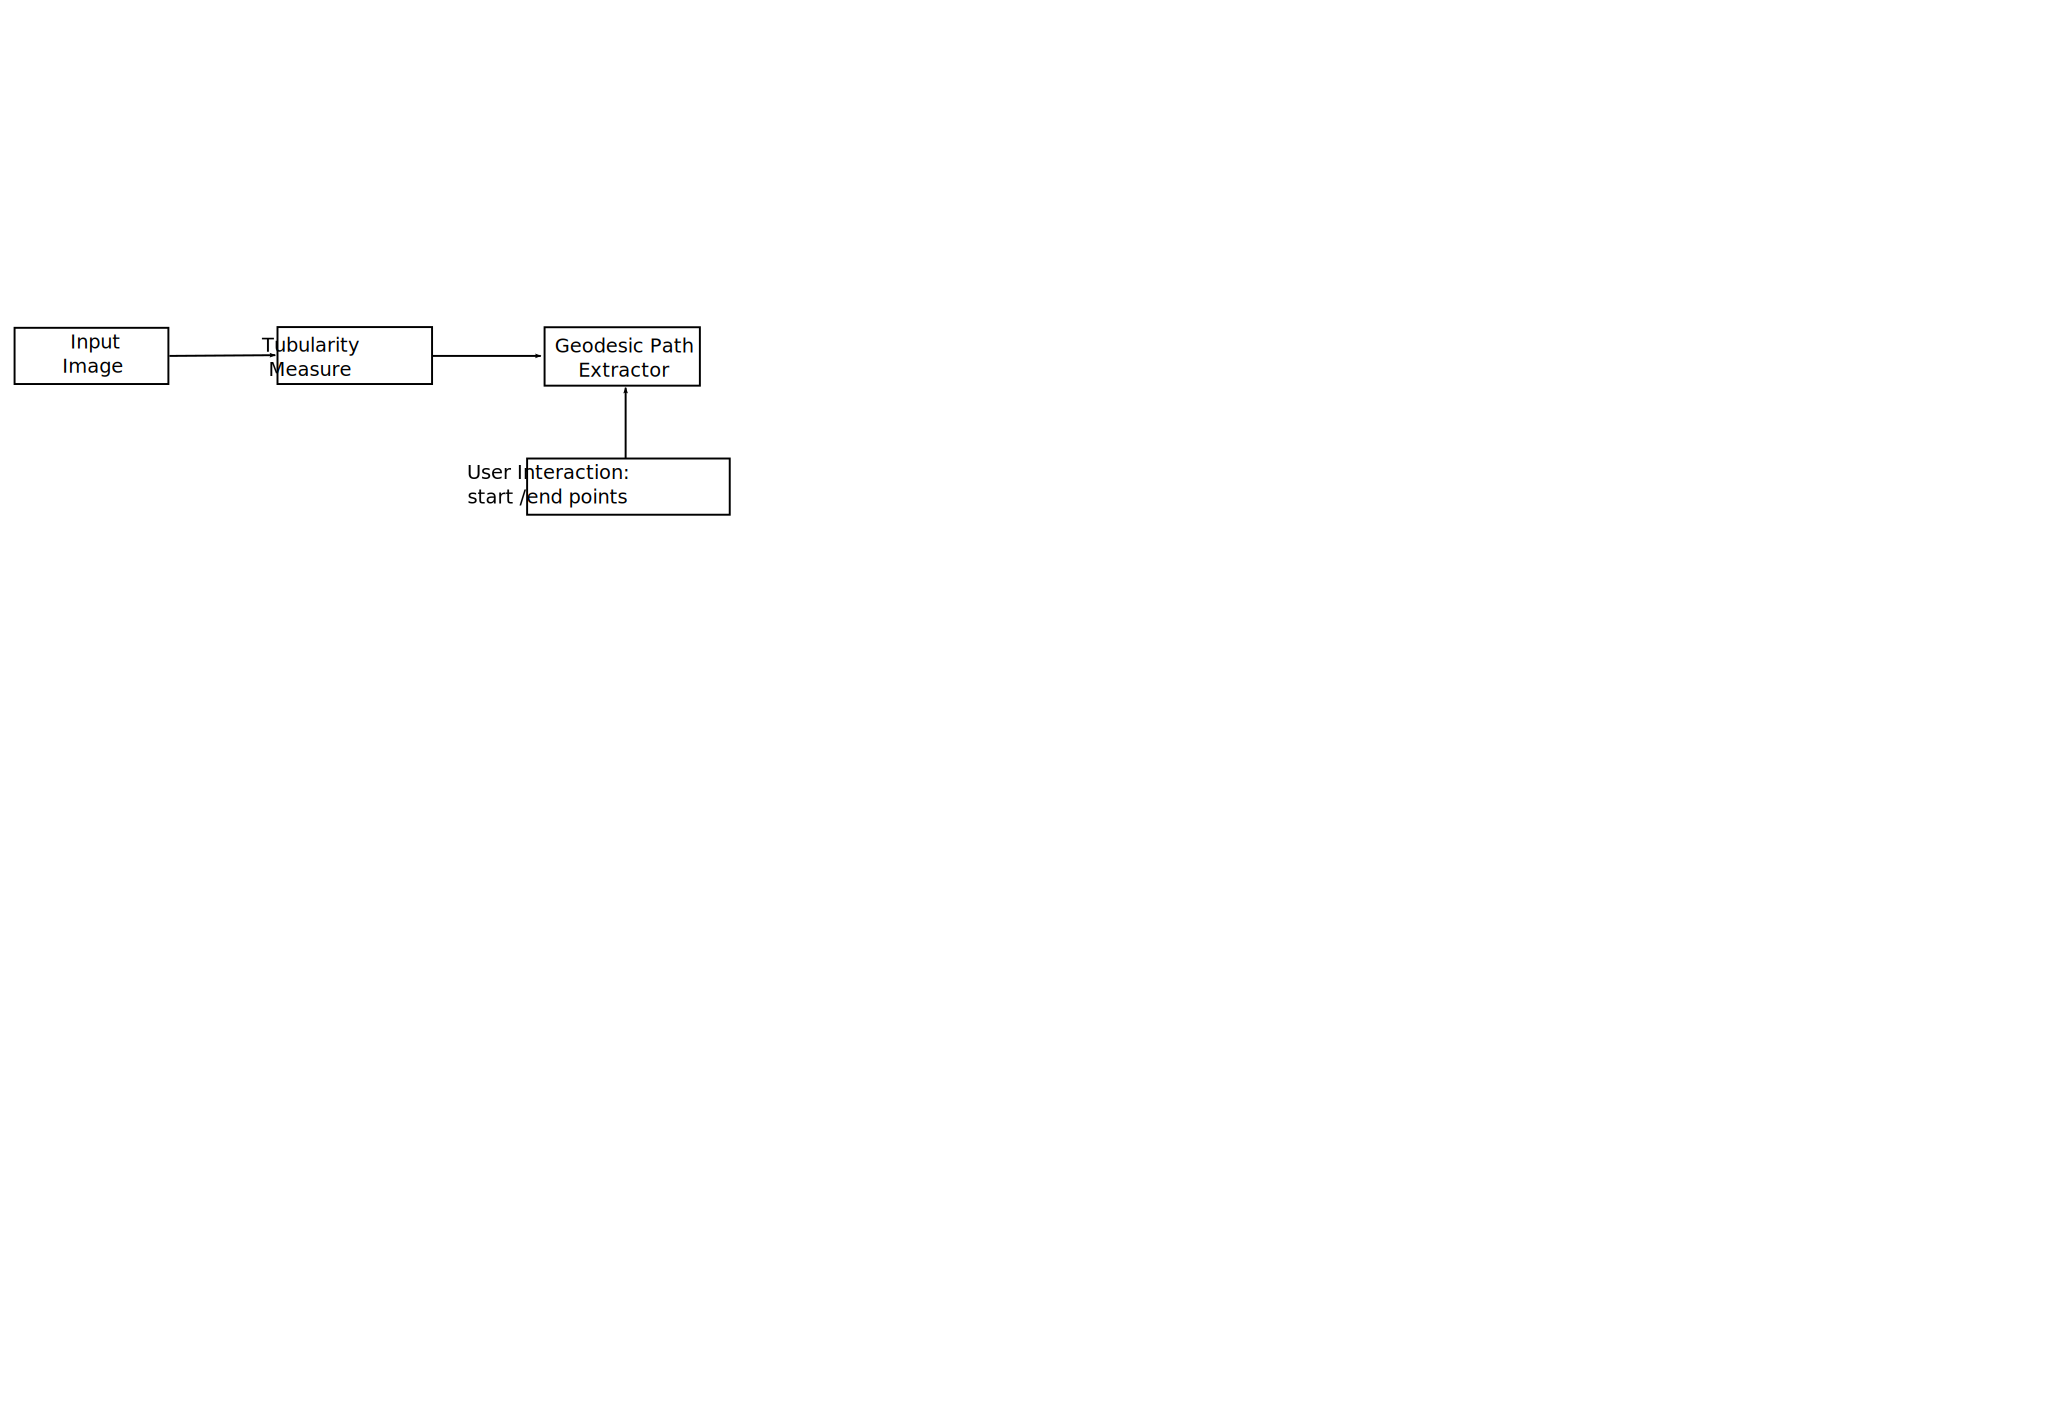
\includegraphics[width=0.5\linewidth]{Diagram}
\end{center}
%Caption
\caption{The tubular geodesic computation pipeline.}
%Caption
\label{fig:diagram}
\end{figure}
%FFFFFFFFFFFFFFFFFFFFFFFFFFFFFFFFFFFFFFFFFFFFFFFFFFFFFFFFFFFFFFFFFFFFFFFFFFFF

Compared to the ITK implementation proposed in~\cite{Mueller2008}, which provides only centreline locations, our method provides, at the same time, radius estimates. Moreover, our back-propagation step uses the $4^{th}$ order Runge-Kutta optimizer, and hence, results in fewer oscillations. Finally, in~\cite{Mueller2008} the author claims that \lq\lq choosing an appropriate speed function is the most difficult part of the entire process\rq\rq. We propose an implementation that provides a well suited speed function to extract tubular structures.

This implementation have been incorporated in the \texttt{ImageJ/FIJI} plugin \textit{Simple Neurite Tracer} \footnote{\url{http://cvlab.epfl.ch/software/delin/index.php}} (SNT) for semi-automatic tracing of curvilinear structures as illustrated in Fig.~\ref{fig:snt}.

%FFFFFFFFFFFFFFFFFFFFFFFFFFFFFFFFFFFFFFFFFFFFFFFFFFFFFFFFFFFFFFFFFFFFFFFFFFFF
\begin{figure}[!h]
\begin{center}		
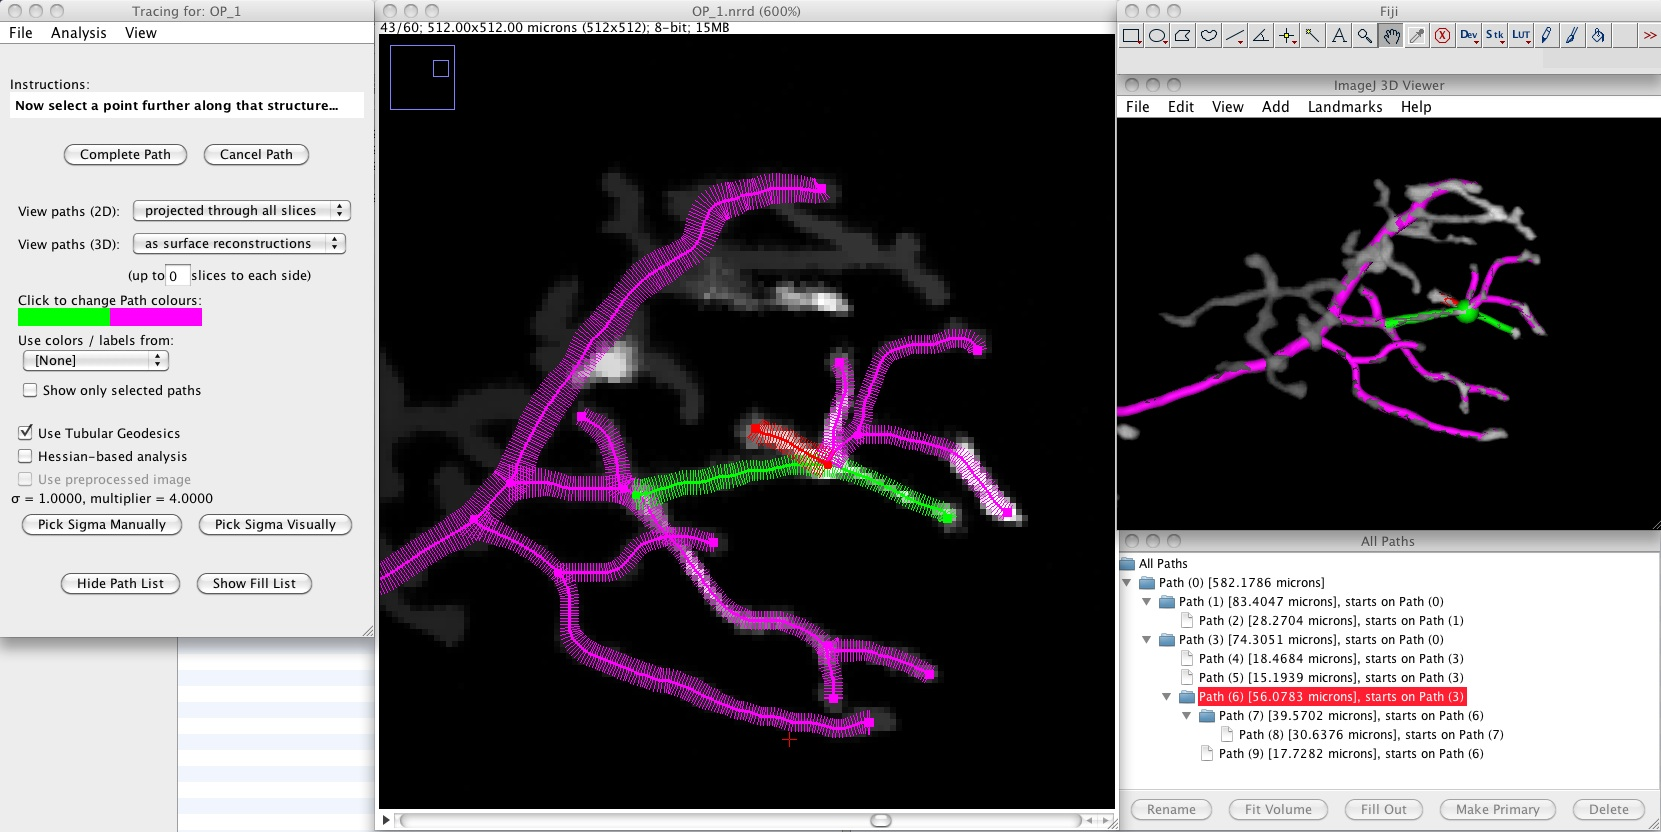
\includegraphics[width=0.70\linewidth]{DemoTubularGeo1}
\end{center}
%Caption
\vspace{-0.5cm}
\caption{Our extended SNT tracer uses the ITK implementation of the method described here.}
%Caption
\label{fig:snt}
\end{figure}
%FFFFFFFFFFFFFFFFFFFFFFFFFFFFFFFFFFFFFFFFFFFFFFFFFFFFFFFFFFFFFFFFFFFFFFFFFFFF


\section{Implementation}

In \cite{Li07}, a variant of the classical, purely spatial, minimal path technique is presented. By incorporating an extra \textit{non-spatial} dimension into the search space, the method models a tubular path in a 3D image as a sequence of 4D points (three spatial dimensions for image coordinates and a scale dimension that quantifies curvilinear structure thickness). Thus, each 4D point represents a sphere in 3D space, and the structure is obtained by taking an envelope of these spheres as we move along a curve (see Fig.~\ref{fig:nDVesselAs} for a 2D example). 

A crucial step of this method is building an informative tubularity measure that drives the propagation. In contrast to the measure used in \cite{Li07}, which requires a few parameters to be tuned, the oriented flux-based measure is parameter free.
%FFFFFFFFFFFFFFFFFFFFFFFFFFFFFFFFFFFFFFFFFFFFFFFFFFFFFFFFFFFFFFFFFFFFFFFFFFFF
\begin{figure}[!h]
\begin{center}		
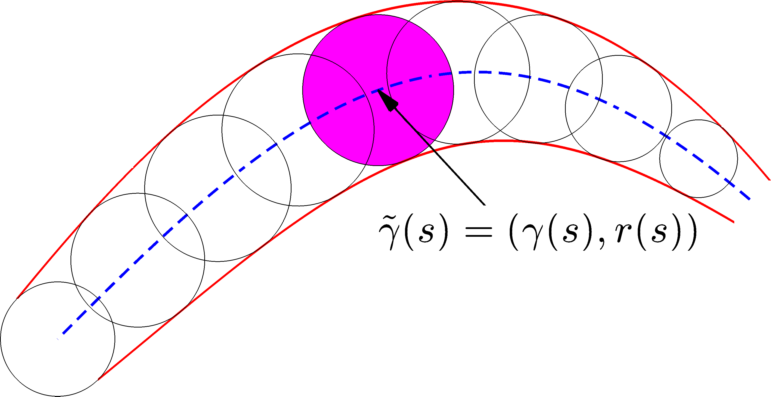
\includegraphics[width=0.5\linewidth]{SynthVessels}
\end{center}
%Caption
\caption{A curvilinear structure is represented as an envelope of a family of cicles with continuously changing center points and radii.}
%Caption
\label{fig:nDVesselAs}
\end{figure}
%FFFFFFFFFFFFFFFFFFFFFFFFFFFFFFFFFFFFFFFFFFFFFFFFFFFFFFFFFFFFFFFFFFFFFFFFFFFF

In the following, we describe our implementation of the oriented flux measure and the tubular geodesic method.

\subsection{Tubularity Measure}

The tubularity measure we use is a function of the OOF matrix \cite{Law08}.
At each image location $\mathbf{x}$, the oriented flux measure is defined as the amount of the image gradient projected 
along a direction $\mathbf{v}$ flowing out from a 3D local sphere (or a 2D circle) $S_r$ centered at the point $\mathbf{x}$. Let $I$ be the image. The OOF measure is defined as
%++++++++++++++++++++++++++++++++++++++++++++++++++++++++++++++++++++++++++++
\begin{equation}
f(\mathbf{x}, \mathbf{v};r)
=\int_{\partial S_r} \left((\nabla (G*I)(\mathbf{x} + \mathbf{h})\cdot \mathbf{v})\mathbf{v}\right)
\cdot \mathbf{n} \mathrm{d}a,
\label{eqn:oflux}
\end{equation}
%++++++++++++++++++++++++++++++++++++++++++++++++++++++++++++++++++++++++++++
where $G$ is a Gaussian function with a sufficiently small standard deviation (typically taken as the minimum image spacing or half of it), $r$ is the radius of the sphere (or circle), $\mathbf{h} = r \mathbf{n}$ is the relative position vector along $\partial S_r$, with $\mathbf{n}$ being the outward unit normal of $\partial S_r$, and $\mathrm{d}a$ is an infinitesimal area (or length) on $\partial S_r$. The function $f$ is the flux of the smoothed image gradient $\nabla(G*I)$ projected along direction $\mathbf{v}$ towards the sphere $\partial S_r$. To detect curvilinear structures having higher intensity values than the background, one would be interested in finding the structure direction at $\mathbf{x}$, which minimizes $f(\mathbf{x}, \mathbf{v}; r)$, i.e. we are looking for
%++++++++++++++++++++++++++++++++++++++++++++++++++++++++++++++++++++++++++++
\begin{equation}
\arg\min\limits_{\mathbf{v}} f(\mathbf{x}, \mathbf{v};r).
\label{eqn:min}
\end{equation}
%++++++++++++++++++++++++++++++++++++++++++++++++++++++++++++++++++++++++++++
Using the divergence theorem, it can be shown that $f(\mathbf{x}, \mathbf{v};r)$ is a quadratic form on $\mathbf{v}$ and its associated matrix can be calculated using a convolution operation,
%++++++++++++++++++++++++++++++++++++++++++++++++++++++++++++++++++++++++++++
\begin{equation}\label{eqn:ofluxmatrix}
f(\mathbf{x}, \mathbf{v};r)= \mathbf{v}^{T}\,\,\left\{ I*(\partial_{i,j} G)*\mathds{1}_{S_r} (\mathbf{x})\right\}\,\, \mathbf{v} := \mathbf{v}^{T}\,\,\left\{ I*\mathbf{F}_r (\mathbf{x})\right\}\,\, \mathbf{v},
\end{equation}
%++++++++++++++++++++++++++++++++++++++++++++++++++++++++++++++++++++++++++++
where $(\partial_{i,j} G)$ is the Hessian matrix of function $G$ and $\mathds{1}_{S_r}$ is the indicator function of the sphere (or circle) $S_r$. $\mathbf{F}_r$ is called the \textit{oriented flux filter}. 

By differentiating the above equation with respect to $\mathbf{v}$, minimization of function $f$ is in turn acquired as solving a generalized eigenvalue decomposition problem. Solving the aforementioned generalized eigen decomposition problem gives $N$ eigenvalues for an N-D image, $\lambda_1(\cdot)\leq \dots\leq \lambda_{N}(\cdot)$. To handle the structures of varying thickness, we follow the multi-scale approach of Law and Chung~\cite{Law08}, which normalizes the  eigenvalues of the OOF matrix by the surface area of the sphere ($4\pi r^2$). In the 2D case, the eigenvalues are normalized by the circle perimeter $2\pi r$.

The normalized convolution $I*\mathbf{F}_r/r^{N-1}$ is performed in the Fourier domain 
for efficiency and implemented in  the \code{itk::OrientedFluxMatrixImageFilter} class.  .
This filter is templated over the input image type and the output image type for which the default pixel type is \code{itk::SymmetricSecondRankTensor}, since the OOF provides a symmetric matrix. The filter \code{itk::MultiScaleTubularityMeasureImageFilter} implements a multi-scale oriented flux measure by summing the $(N-1)$ eigenvalues of the OOF matrix that correspond to the cross-section of the tubular structures. In addition to the  (N+1)-D tubularity measure, the filter optionally outputs scale and OOF matrix images. See \code{itkMultiScaleTubularityMeasureImageFilter.cxx} for a complete example.

\subsection{Tubular Geodesic}
A \textit{tubular geodesic} is a path, linking two points, that globally minimizes an energy functional of the tubularity measure. Without loss of generality and in order to simplify notations we will assume hereinafter that a path $\gamma$ is parametrized along its length $s$ ($0 \leq s \leq 1$). The energy minimized by a geodesic is under the form:
%++++++++++++++++++++++++++++++++++++++++++++++++++++++++++++++++++++++++++++
\begin{equation}\label{eqn:IsotropicEnergy}
E(\gamma)=\int \mathcal{P}\big( \gamma(s) \big)\mathrm{d}s.
\end{equation}
%++++++++++++++++++++++++++++++++++++++++++++++++++++++++++++++++++++++++++++
where $\mathcal{P(\mathbf{x})} > 0$ is the tubularity measure described in the previous section.

For an N-D image, a geodesic path connecting two (N+1)-D points $\mathbf{p}_{1}$ and $\mathbf{p}_{2}$, globally 
minimizes the above energy (\ref{eqn:IsotropicEnergy}) and is noted as $\mathcal{C}_{\mathbf{p}_{1},\mathbf{p}_{2}}$.

The solution of this minimization problem is obtained through the computation of the \textit{geodesic distance} $\mathcal{U}:\Omega\rightarrow\mathbb{R}^{+}$ associated with~$\mathbf{p}_{1}$ on the domain $\Omega\subset\mathbb{R}^N$. The geodesic distance is the minimal energy integrated along a path between $\mathbf{p}_{1}$ and any point $\mathbf{x}$ of the domain $\Omega$ :
%++++++++++++++++++++++++++++++++++++++++++++++++++++++++++++++++++++++++++++
\begin{equation}\label{eqn:minimalactionmap1}
\forall~\mathbf{x}\in\Omega,~\mathcal{U}(\mathbf{x})=
\min_{\gamma \in \mathcal{A}_{\mathbf{p}_{1},\mathbf{x}}}
\Bigg\{ \int \mathcal{P}\big(\gamma(s) \big) \mathrm{d}s \Bigg\}~,
\end{equation}
%++++++++++++++++++++++++++++++++++++++++++++++++++++++++++++++++++++++++++++
where $\mathcal{A}_{\mathbf{p}_{1},\mathbf{x}}$ is the set of paths connecting $\mathbf{x}$ to $\mathbf{p}_{1}$.
The values of $\mathcal{U}$ may be regarded as the arrival times of a front propagating 
from the source $\mathbf{p}_{1}$ with velocity  $1/\mathcal{P}$.
$\mathcal{U}$ satisfies the Eikonal equation
%++++++++++++++++++++++++++++++++++++++++++++++++++++++++++++++++++++++++++++
\begin{equation}\label{eqn:eikonal1}
\|\nabla \mathcal{U}(\mathbf{x})\| =  \mathcal{P(\mathbf{x})} \; \; \; \; \; \; \; \forall~\mathbf{x}\in\Omega,\text{ and }   \mathcal{U}(\mathbf{p}_{1}) = 0,
\end{equation}
%++++++++++++++++++++++++++++++++++++++++++++++++++++++++++++++++++++++++++++
The map $\mathcal{U}$ has only one global minimum, the source point $\mathbf{p}_{1}$, and its flow lines satisfy the Euler-Lagrange equation of functional (\ref{eqn:IsotropicEnergy}). Therefore, the minimal energy path $\mathcal{C}_{\mathbf{p}_{1},\mathbf{p}_{2}}$ can be retrieved with a simple gradient descent on $\mathcal{U}$ from $\mathbf{p}_{2}$ to $\mathbf{p}_{1}$ by solving the following ordinary differential equation with standard numerical methods such as Heun's or Runge-Kutta's methods.
%++++++++++++++++++++++++++++++++++++++++++++++++++++++++++++++++++++++++++++
\begin{equation}\label{eqn:gradientdescent1}
\displaystyle\frac{\mathrm{d} \mathcal{C}_{\mathbf{p}_{1},\mathbf{p}_{2}}}{\mathrm{d}s} (s) \propto 
 -\nabla\mathcal{U}\big(\mathcal{C}_{\mathbf{p}_{1},\mathbf{p}_{2}}(s)\big),\text{ with }\mathcal{C}_{\mathbf{p}_{1},\mathbf{p}_{2}}(0) = \mathbf{p}_{1}  \text{ and }\mathcal{C}_{\mathbf{p}_{1},\mathbf{p}_{2}}(1) = \mathbf{p}_{2}.
\end{equation}
%++++++++++++++++++++++++++++++++++++++++++++++++++++++++++++++++++++++++++++

The filter class that computes a geodesic path from a given tubularity image is \code{itk::TubularMetricToPathFilter}, which is a subclass of \code{itk::ImageToPathFilter}. The filter expects one start point, a set of end points, and an (N+1)-D tubularity image to drive the front propagation. The tubularity image must be a scalar one with real and strictly positive pixel values. 

The front propagation step is carried out using the ITK filter class \code{itk::FastMarchingUpwindGradientImageFilter}. The back-propagation can be  performed using a 
discrete neighborhood iterator, \code{itk::IterateNeighborhoodCharacteristicDirectionsToPathFilter} for discrete centreline location and radius estimates, or a fixed step 
gradient descent optimizer, \code{itk::FixedStepDescentCharacteristicDirectionsToPathFilter} for sub-pixel accuracy, similar to the ones proposed in \cite{Mueller2008}. 
However, both of these approaches result in oscillations along path centerlines especially when the curvilinear structures are faint and the image is noisy. To achieve 
robustness against  these factors, we implemented the $4^{th}$ order Runge-Kutta back propagation filter \code{itk::RK4CharacteristicDirectionsToPathFilter}. 

%
%For the implementation, first describe quickly \code{PolyLineParametricTubularPath}.
%Second, recall that equation (\ref{eqn:eikonal1}) is solved using the fast marching algorithm
%\listcpluspluspsnip
%\lstinputlisting[float,label=typedef:FM,linerange={89-92}]
%                 {../src/itkTubularMetricToPathFilter.h}
%                 
%\listcpluspluspsnip                 
%\lstinputlisting[float,label=lst:Slice1,linerange={229-231,240-249,251-267}]
%                 {../src/itkTubularMetricToPathFilter.hxx}
%
%The implementation of the geodesic path extractor consists of one filter 
%\listcpluspluspsnip
%\lstinputlisting[float,label=lst:Slice1,linerange={259-261}]
%                 {../src/itkTubularMetricToPathFilter.cxx}
%
%In this project, we implemented a number of auxiliary functions and filters, nevertheless only two filters are expected to be used:
%\begin{itemize}
%\item[$\bullet$] \code{itk::MultiScaleOrientedFluxBasedMeasureFFTImageFilter}
%\item[$\bullet$] \code{itk::TubularMetricToPathFilter}
%\end{itemize}



\section{Examples}

%FFFFFFFFFFFFFFFFFFFFFFFFFFFFFFFFFFFFFFFFFFFFFFFFFFFFFFFFFFFFFFFFFFFFFFFFFFFF
\begin{figure}[t]
  \centering
  \begin{tabular}{ccc}
    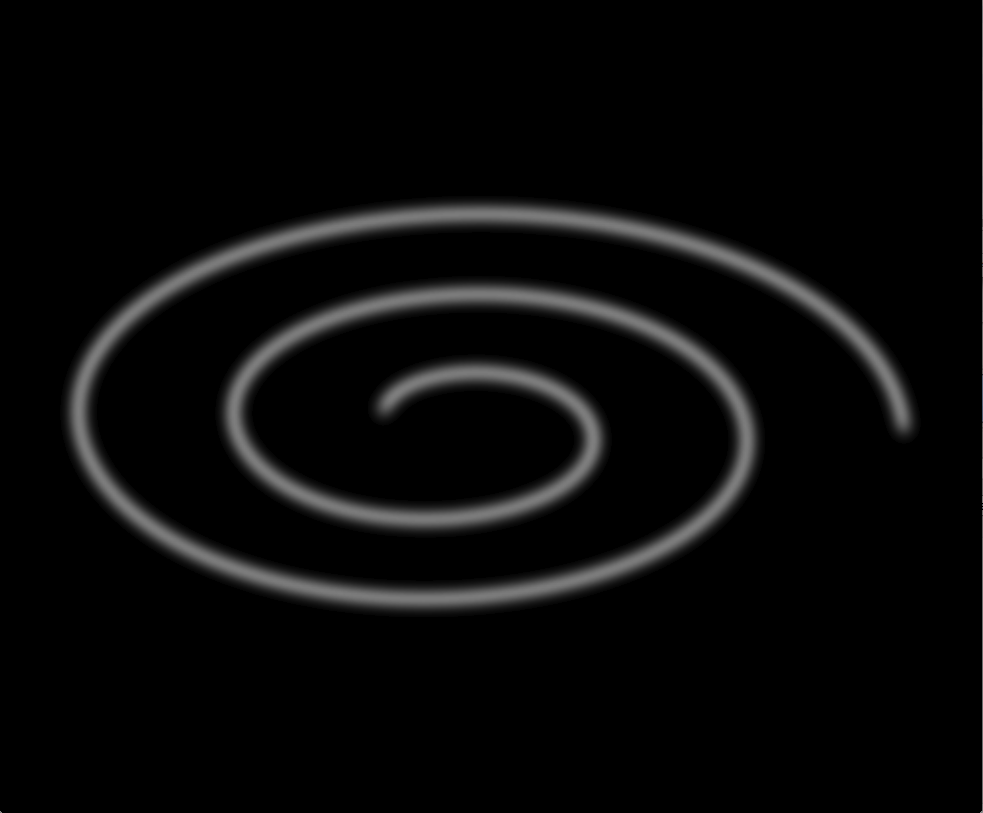
\includegraphics[height=0.31\columnwidth, width=0.31\columnwidth]{Synthetic-02.png} &
    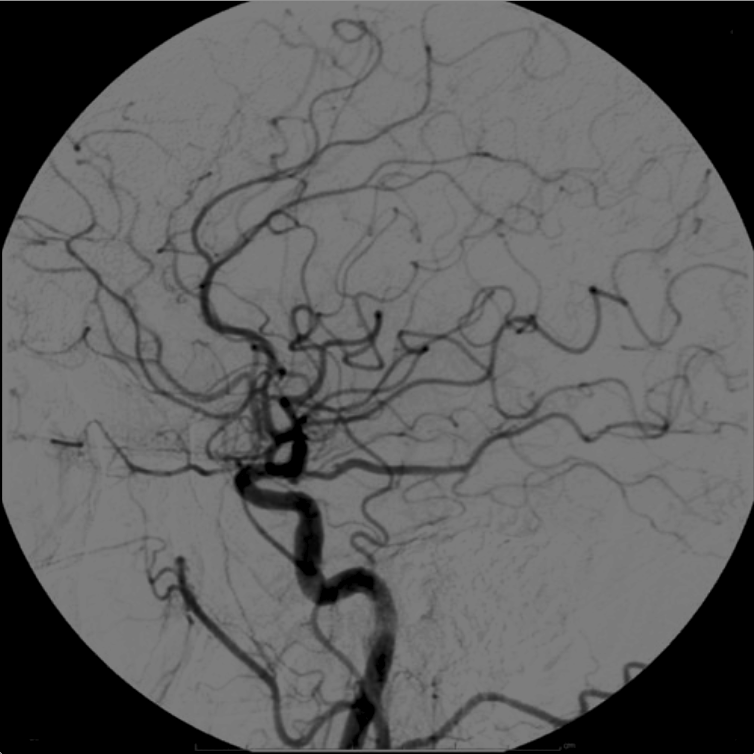
\includegraphics[width=0.31\columnwidth]{Real-DSA-01.png} &
    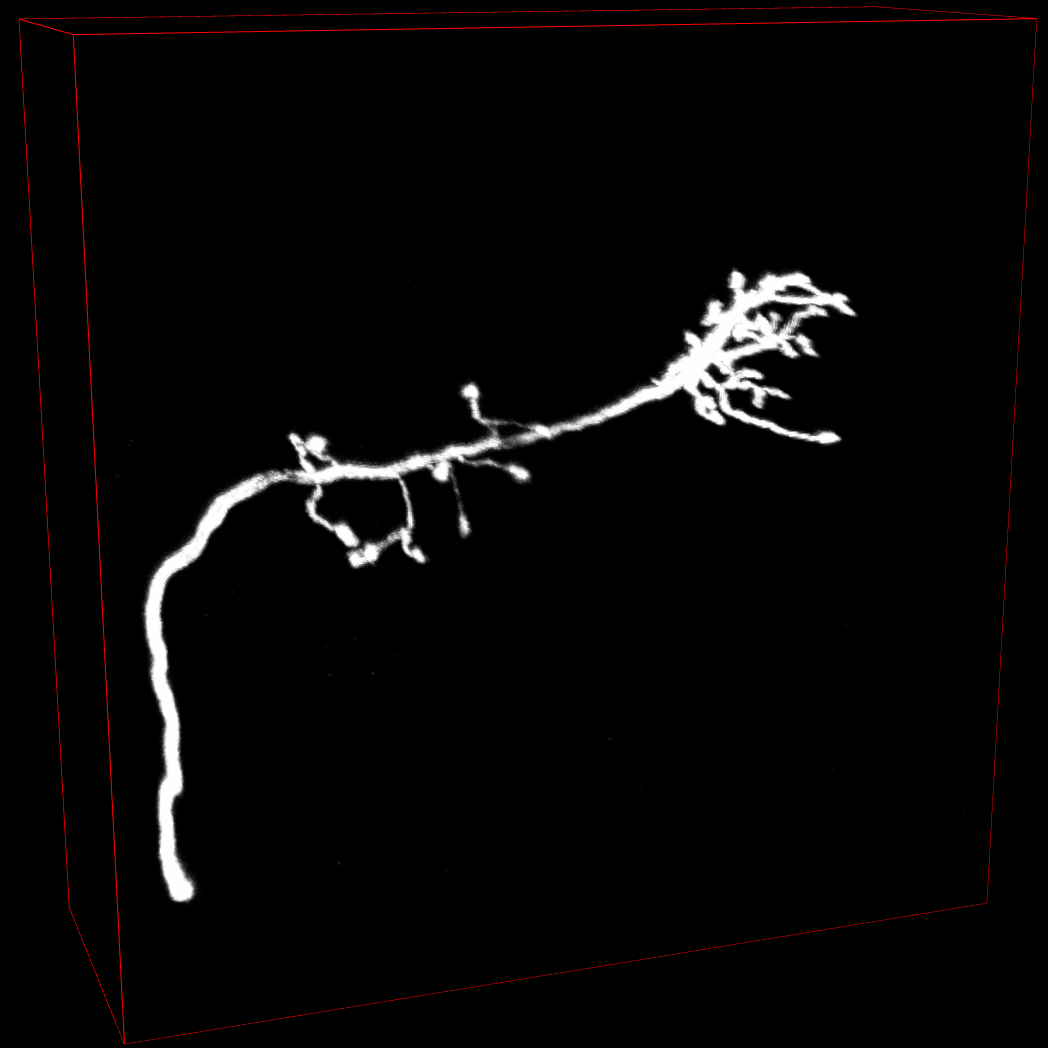
\includegraphics[width=0.31\columnwidth]{OP_1_3D.png} \\
    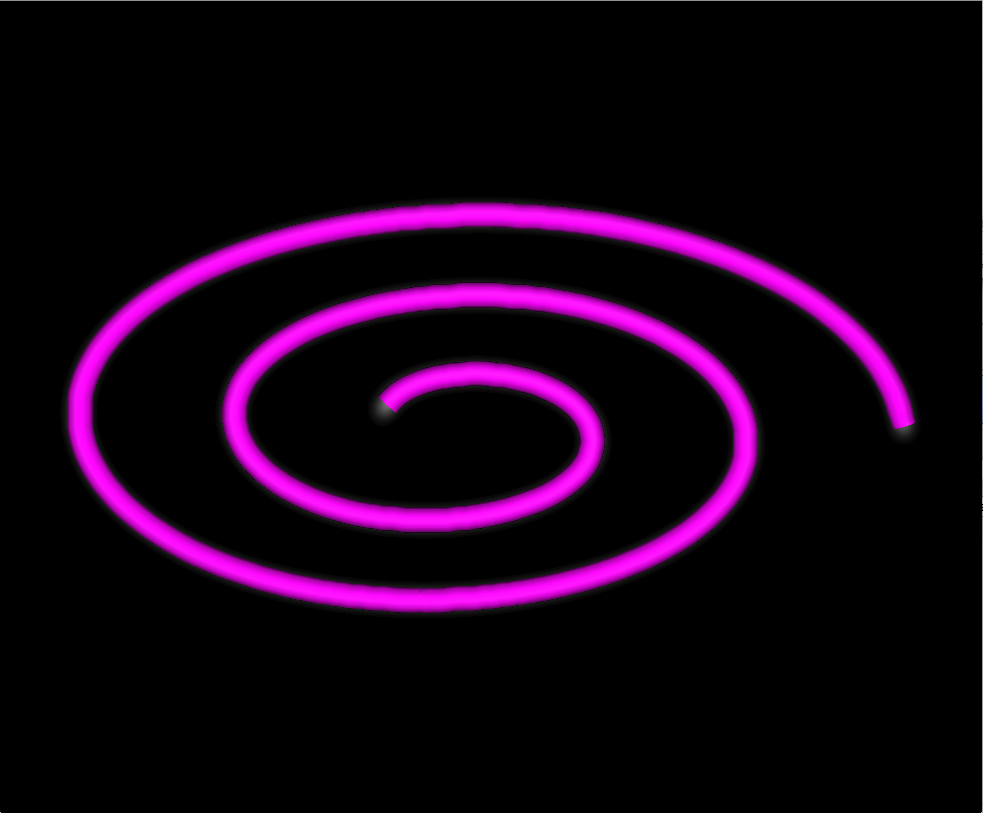
\includegraphics[height=0.31\columnwidth, width=0.31\columnwidth]{Synthetic-02_reconst.png} &
    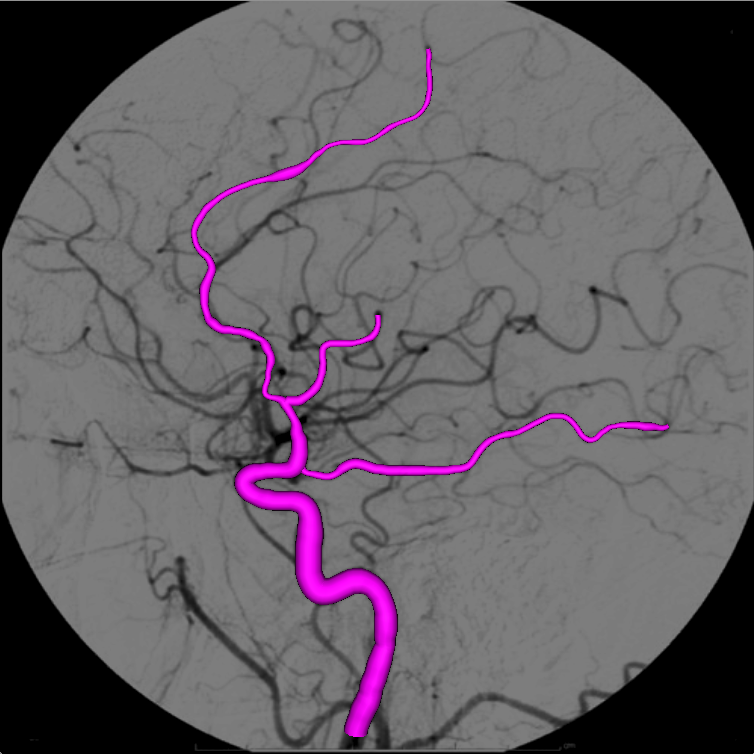
\includegraphics[width=0.31\columnwidth]{Real-DSA-01_reconst.png} &
    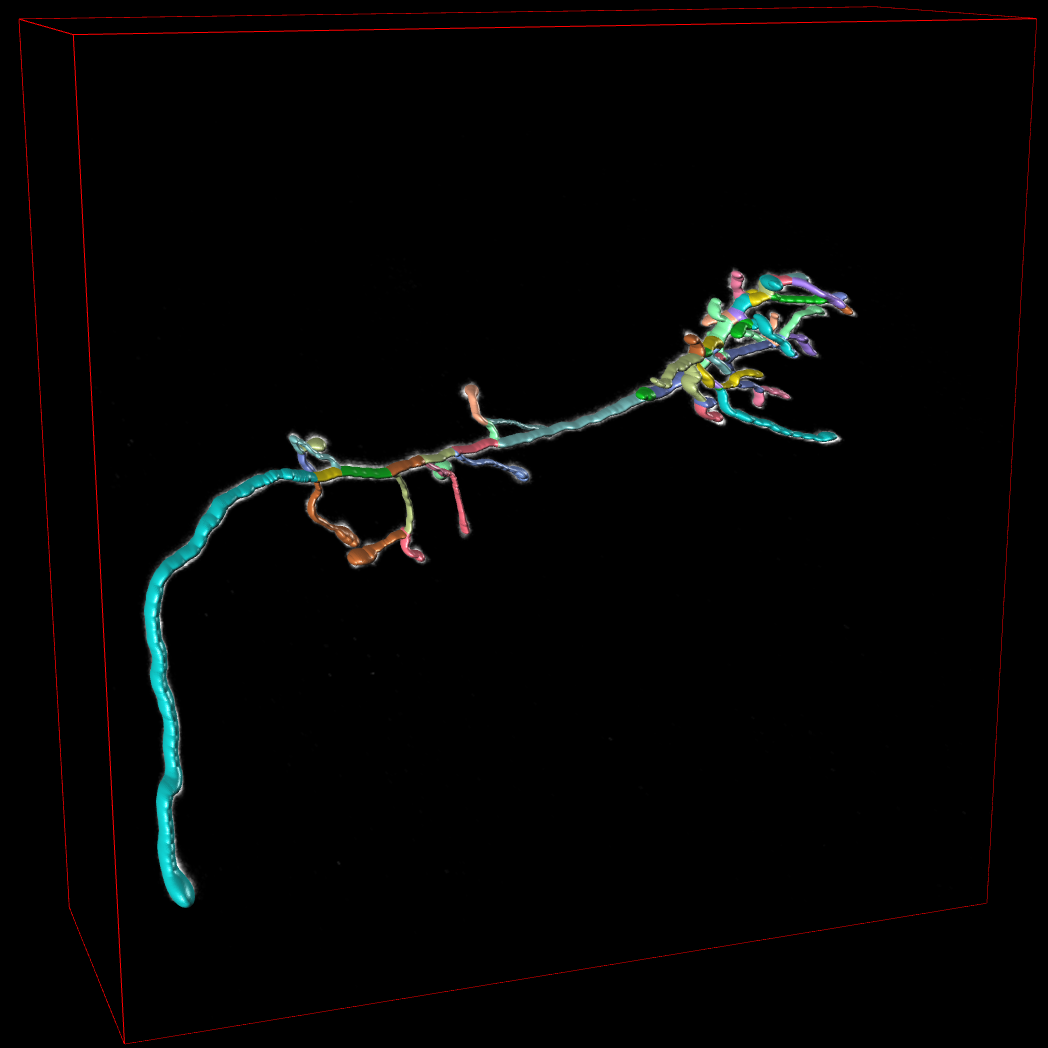
\includegraphics[width=0.31\columnwidth]{OP_1_reconst_3D.png}  \\
  \end{tabular}
  \caption{  \label{fig:results} First row: from left to right, a synthetically generated image containing a 
  spiral shape, a 2D cerebral angiogram, a 3D stack of olfactory projection fibers  (OP) from the DIADEM  
  competition \cite{Diadem10}. Second row: tracing results overlaid on top of the images. Each branch in the 
  structures is traced by manually providing a start and an end point. The reconstruction for the OP stack is 
  color coded for easier visibility.}
  \vspace{-0.3cm}
\end{figure}
%FFFFFFFFFFFFFFFFFFFFFFFFFFFFFFFFFFFFFFFFFFFFFFFFFFFFFFFFFFFFFFFFFFFFFFFFFFFF

We've evaluated our pipeline on a large variety of noisy 2D images and 3D images stacks. 
Figure~\ref{fig:results} shows three sample results on a synthetically generated image, a 2D cerebral 
angiogram and a 3D stack of neurite fibers. Maximum intensity projections of the tubularity stacks for 
each scale level are shown in Fig.~\ref{fig:mip_tubularity_images}. 

In the following, we give an example usage of the tubularity and geodesic computation steps for the 3D 
stack shown in Fig.~\ref{fig:results}.

%FFFFFFFFFFFFFFFFFFFFFFFFFFFFFFFFFFFFFFFFFFFFFFFFFFFFFFFFFFFFFFFFFFFFFFFFFFFF
\begin{figure}[t]
  \centering
  \begin{tabular}{ccc}
    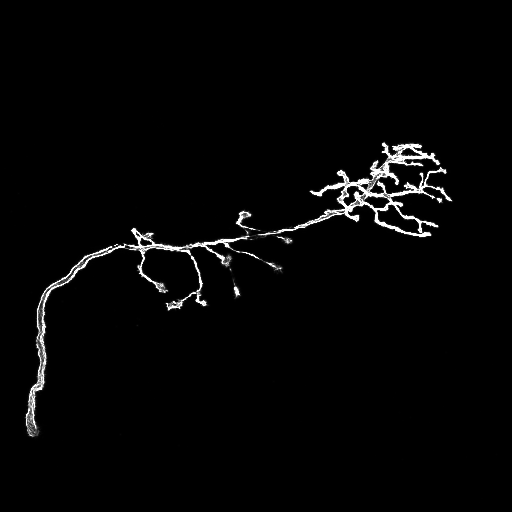
\includegraphics[width=0.31\columnwidth]{OP_1_01_max_scale_space_tubularity.png} &
    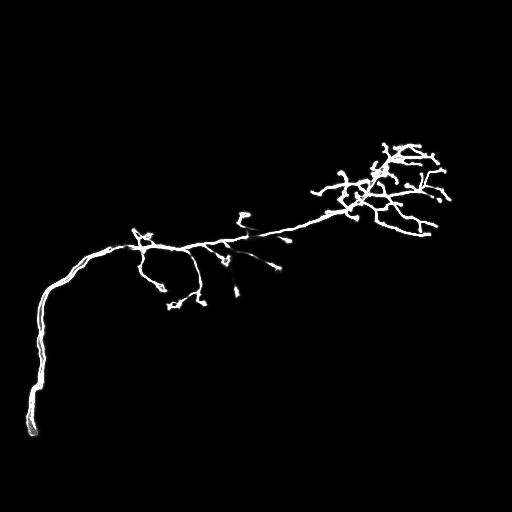
\includegraphics[width=0.31\columnwidth]{OP_1_03_max_scale_space_tubularity.png} &
    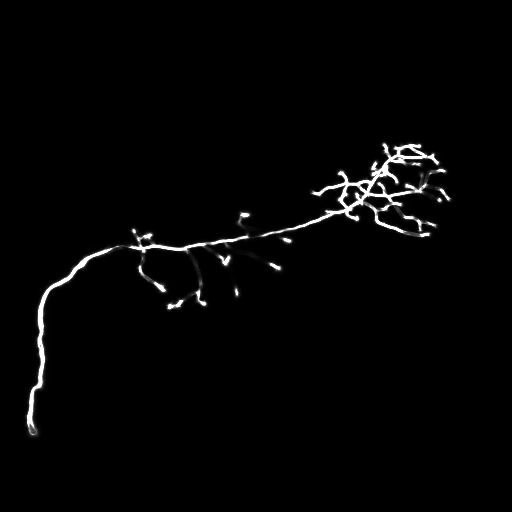
\includegraphics[width=0.31\columnwidth]{OP_1_05_max_scale_space_tubularity.png} \\
    $r = 1.0$ & $r = 2.0$ & $r = 3.0$ \\ \\
    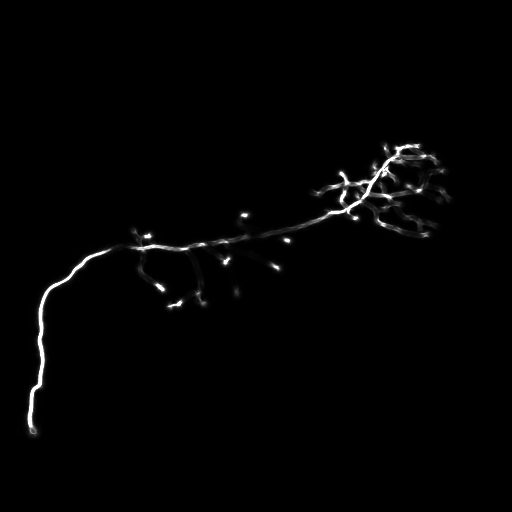
\includegraphics[width=0.31\columnwidth]{OP_1_07_max_scale_space_tubularity.png} &
    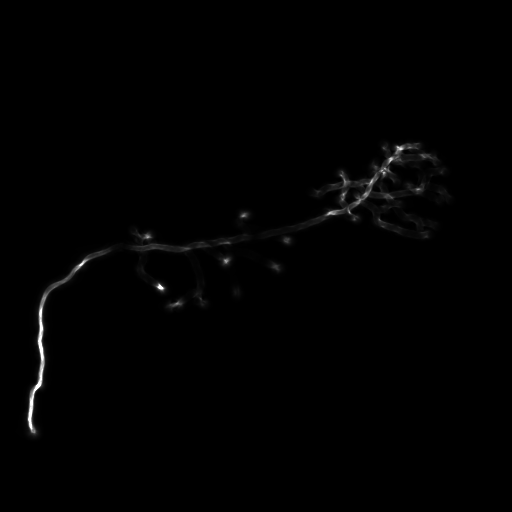
\includegraphics[width=0.31\columnwidth]{OP_1_09_max_scale_space_tubularity.png} &
    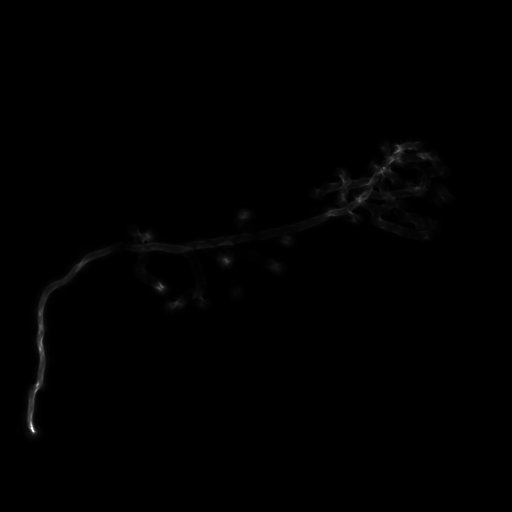
\includegraphics[width=0.31\columnwidth]{OP_1_11_max_scale_space_tubularity.png}  \\
    $r = 4.0$ & $r = 5.0$ & $r = 6.0$ \\
  \end{tabular}
  \caption{  \label{fig:mip_tubularity_images} Maximum intensity projections of the computed 
  tubularity volumes for the OP stack shown in the last column of Fig.~\ref{fig:results}. 
  Each image corresponds to a different radius level $r$, which is given below it.}
  \vspace{-0.3cm}
\end{figure}
%FFFFFFFFFFFFFFFFFFFFFFFFFFFFFFFFFFFFFFFFFFFFFFFFFFFFFFFFFFFFFFFFFFFFFFFFFFFF

\listcpluspluspsnip
\lstinputlisting{example_code.cxx}

\section{Conclusion}

In this work, we've presented an ITK framework for computing tubular geodesics from point pairs. The 
framework allows a user to first generate a scale-space tubularity volume with 
the curvilinear structures enhanced  and the background noise suppressed. This volume is then used 
as a speed function to compute a tubular geodesic for each start and end point pair, which is done using 
the fast marching algorithm and the $4^{th}$ order Runge-Kutta gradient descent procedure. This results 
in a generic and efficient method to trace curvilinear structures in medical imagery.

\bibliographystyle{plain}
\bibliography{TubularGeodesicITK}


\end{document}
